\documentclass[10.5pt]{article}
\usepackage[a4paper,margin=15mm,headheight=23pt]{geometry}
\usepackage{lmodern}
\usepackage[T1]{fontenc}
\usepackage{microtype}
\usepackage{amsmath,amssymb,mathtools}
\usepackage{xcolor}
\usepackage{tikz}
\usepackage{tcolorbox}
\usepackage{booktabs,array}
\usepackage{fancyhdr}
\usepackage{enumitem}
\usepackage{hyperref}
\usepackage{lastpage}
\definecolor{ink}{HTML}{172232}\definecolor{blue}{HTML}{2D5BFF}\definecolor{cyan}{HTML}{0B8E91}\definecolor{orange}{HTML}{E8743B}\definecolor{paper}{HTML}{F6F5F0}\definecolor{mist}{HTML}{EEF1F5}\definecolor{line}{HTML}{D7DCE3}
\pagecolor{paper}\color{ink}\hypersetup{colorlinks=true,linkcolor=blue,urlcolor=blue}
\pagestyle{fancy}\fancyhf{}\lhead{\textsf{Multivariable Taylor cheat sheet}}\rhead{\textsf{Series Lab}}\cfoot{\textsf{\thepage\,/\,\pageref{LastPage}}}\renewcommand{\headrulewidth}{.4pt}\renewcommand{\headrule}{\hbox to\headwidth{\color{line}\leaders\hrule height \headrulewidth\hfill}}
\newtcolorbox{bluebox}[1][]{colback=blue!6,colframe=blue!55!ink,boxrule=.5pt,arc=4pt,left=7pt,right=7pt,top=5pt,bottom=5pt,#1}
\newtcolorbox{orangebox}[1][]{colback=orange!7,colframe=orange!65!ink,boxrule=.5pt,arc=4pt,left=7pt,right=7pt,top=5pt,bottom=5pt,#1}
\newtcolorbox{graybox}[1][]{colback=mist,colframe=line,boxrule=.5pt,arc=4pt,left=7pt,right=7pt,top=5pt,bottom=5pt,#1}
\newcommand{\tagline}[1]{\par\medskip\textcolor{blue}{\sffamily\footnotesize\bfseries #1}\par\vspace{1pt}}
\begin{document}
\thispagestyle{empty}
{\sffamily\footnotesize\bfseries\textcolor{blue}{SERIES LAB\hspace{7pt}/\hspace{7pt} MULTIVARIABLE CALCULUS}}\\[-1pt]
{\fontsize{27}{30}\selectfont\bfseries Multivariable Taylor polynomials}\par
{\large\color{cyan}A calculation-first cheat sheet for approximating functions of several variables}\par\vspace{4mm}
\begin{bluebox}
\textbf{The one-line idea.} Near $a\in\mathbb R^n$, replace $f(a+h)$ by a polynomial in the displacement $h=x-a$. The gradient supplies the linear part; the Hessian supplies curvature.
\[
\boxed{\displaystyle T_2(a+h)=f(a)+\nabla f(a)^T h+\frac12h^T H_f(a)h}\qquad\text{and}\qquad f(a+h)=T_2(a+h)+\mathcal O(\|h\|^3).
\]
\end{bluebox}
\tagline{01 / THE WORKFLOW}
\begin{enumerate}[leftmargin=*,itemsep=2pt,topsep=2pt]
\item \textbf{Choose the centre:} write $a=(a_1,\ldots,a_n)$ and $h=x-a$.
\item \textbf{Evaluate the function:} compute $f(a)$.
\item \textbf{Evaluate first derivatives:} compute $\nabla f(a)=\bigl(f_{x_1}(a),\ldots,f_{x_n}(a)\bigr)$.
\item \textbf{Evaluate second derivatives:} form the Hessian $H_f(a)=[f_{x_ix_j}(a)]$.
\item \textbf{Assemble:} use $f(a)+\nabla f(a)^Th+\tfrac12h^TH_f(a)h$.
\item \textbf{State the remainder and domain:} degree $2$ means error $\mathcal O(\|h\|^3)$; scalar prototypes may add conditions such as $|u|<1$.
\item \textbf{Check one point:} compare $T_2$ with $f$ numerically.
\end{enumerate}
\tagline{02 / FORMULAS TO MEMORISE}
\begin{center}
\renewcommand{\arraystretch}{1.25}
\begin{tabular}{>{\raggedright\arraybackslash}p{.28\linewidth} p{.63\linewidth}}
\toprule
\textbf{Object} & \textbf{Formula}\\\midrule
First order & $T_1=f(a)+\nabla f(a)^T h$\\
Second order & $T_2=f(a)+\nabla f(a)^T h+\frac12h^TH_f(a)h$\\
Two variables & $\frac12h^THh=\frac12(f_{xx}u^2+2f_{xy}uv+f_{yy}v^2)_a$\\
Degree $m$ & $\displaystyle T_m(a+h)=\sum_{|\alpha|\le m}\frac{D^\alpha f(a)}{\alpha!}h^\alpha$\\
Remainder & $f(a+h)-T_m(a+h)=\mathcal O(\|h\|^{m+1})$\\
\bottomrule
\end{tabular}
\end{center}
\begin{graybox}
\textbf{Multi-index key.} $\alpha=(\alpha_1,\ldots,\alpha_n)$, $|\alpha|=\sum_i\alpha_i$, $\alpha!=\prod_i\alpha_i!$, $D^\alpha f=\partial_1^{\alpha_1}\cdots\partial_n^{\alpha_n}f$, and $h^\alpha=\prod_i h_i^{\alpha_i}$. 
\end{graybox}
\tagline{03 / SINGLE-VARIABLE WORKED EXAMPLES}
\textbf{Example 1: a polynomial.} For $p(t)=3t^2-2t+1$ about $t=1$, let $h=t-1$. Then $p(1)=2$, $p'(1)=4$, and $p''(1)=6$, so
\[
\boxed{T_2(t)=2+4h+3h^2.}
\]
Because $p$ has degree $2$, this is exact: $p(t)=T_2(t)$ everywhere.

\textbf{Example 2: an exponential.} About $t=0$, $e^t$ has derivatives all equal to $1$:
\[
\boxed{T_3(t)=1+t+\frac{t^2}{2}+\frac{t^3}{6}},\qquad R_3=\mathcal O(t^4).
\]
At $t=0.2$, $T_3=1.221333\ldots$ while $e^{0.2}=1.221403\ldots$.

\textbf{Example 3: a convergence condition.} From $\ln(1+t)=t-t^2/2+t^3/3+\cdots$,
\[
\boxed{T_3(t)=t-\frac{t^2}{2}+\frac{t^3}{3}},\qquad |t|<1.
\]
The radius condition belongs beside the polynomial; it is not optional bookkeeping.

\textbf{Example 4: a geometric series.} Since $(1-t)^{-1}=1+t+t^2+t^3+\cdots$,
\[
\boxed{T_3(t)=1+t+t^2+t^3},\qquad |t|<1.
\]
\tagline{04 / FIRST MULTIVARIABLE EXAMPLE}
For $f(x,y)=e^{x+y}$ about $a=(0,0)$, every first and second partial derivative equals $e^{x+y}$, so
\[
f(a)=1,\qquad \nabla f(a)=\begin{pmatrix}1\\1\end{pmatrix},\qquad H_f(a)=\begin{pmatrix}1&1\\1&1\end{pmatrix}.
\]
With $h=(x,y)$,
\[
\boxed{T_2(x,y)=1+x+y+\frac12(x^2+2xy+y^2)=1+x+y+\frac12(x+y)^2.}
\]
At $(x,y)=(0.1,0.2)$: $T_2=1.345$, whereas $e^{0.3}=1.3498588\ldots$; the absolute error is about $4.86\times10^{-3}$.
\vfill
\begin{center}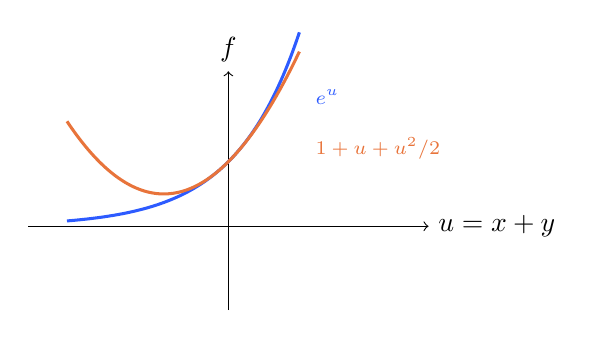
\begin{tikzpicture}[scale=.82]
\draw[->] (-3.1,0)--(3.1,0) node[right] {$u=x+y$};
\draw[->] (0,-1.3)--(0,2.4) node[above] {$f$};
\draw[blue,line width=1.1pt] plot[smooth,domain=-2.5:1.1,samples=100] (\x,{exp(\x)});
\draw[orange,line width=1.1pt] plot[smooth,domain=-2.5:1.1,samples=100] (\x,{1+\x+\x*\x/2});
\node[font=\sffamily\scriptsize,blue,anchor=west] at (1.2,2.0) {$e^u$};\node[font=\sffamily\scriptsize,orange,anchor=west] at (1.2,1.2) {$1+u+u^2/2$};
\end{tikzpicture}\end{center}

\newpage
\tagline{05 / BASIC MULTIVARIABLE WORKED EXAMPLES}
\textbf{Example 1: a quadratic is already its Taylor polynomial.} Let $f(x,y)=x^2+3xy+y^2$ about $(0,0)$. Since $f$ has degree $2$,
\[
\nabla f(0,0)=(0,0),\qquad H_f(0,0)=\begin{pmatrix}2&3\\3&2\end{pmatrix},
\]
so $\boxed{T_2(x,y)=x^2+3xy+y^2=f(x,y)}$. The remainder is exactly zero.

\textbf{Example 2: a linear approximation.} For $f(x,y)=\sqrt{x+y}$ about $(1,1)$, write $u=x-1$, $v=y-1$. Since $f(a)=\sqrt2$ and $\nabla f(a)=(1/(2\sqrt2),1/(2\sqrt2))$,
\[
\boxed{T_1(x,y)=\sqrt2+\frac{u+v}{2\sqrt2}.}
\]
At $(1.02,0.97)$, $(u,v)=(0.02,-0.03)$ and $T_1=1.41068$; the exact value is $\sqrt{1.99}=1.41067\ldots$.

\textbf{Example 3: a vanishing quadratic term.} For $f(x,y)=\sin(x+y)$ about $(0,0)$, set $u=x+y$. Since $\sin u=u-u^3/6+\cdots$,
\[
\boxed{T_2(x,y)=x+y,\qquad f(x,y)-T_2(x,y)=\mathcal O(\|(x,y)\|^3).}
\]
\tagline{06 / INTERMEDIATE MULTIVARIABLE WORKED EXAMPLES}
\textbf{Example 4: a shifted logarithm.} For $f(x,y)=\ln(x+y)$ about $(1,1)$, let $u=x-1$, $v=y-1$. Then
\[
\ln(x+y)=\ln(2+u+v)=\ln2+\frac{u+v}{2}-\frac{(u+v)^2}{8}+\mathcal O(\|(u,v)\|^3),
\]
so $\boxed{T_2=\ln2+(u+v)/2-(u+v)^2/8}$. The condition is $|u+v|<2$.

\textbf{Example 5: reciprocal with cross terms.} For $f(x,y)=1/(1-x-y)$ about $(0,0)$, use $(1-s)^{-1}=1+s+s^2+s^3+\cdots$ with $s=x+y$:
\[
\boxed{T_3=1+(x+y)+(x+y)^2+(x+y)^3.}
\]
Expanded, the cubic part is $x^3+3x^2y+3xy^2+y^3$. The convergence condition is $|x+y|<1$.

\tagline{07 / WORKED EXAMPLE: A NONZERO CENTRE}
Let $f(x,y)=x^2e^y$ and expand about $a=(1,0)$. Use displacement variables $u=x-1$ and $v=y$.
\begin{align*}
f(1,0)&=1, & \nabla f(1,0)&=\begin{pmatrix}2\\1\end{pmatrix}, &
H_f(1,0)&=\begin{pmatrix}2&2\\2&1\end{pmatrix}.
\end{align*}
The quadratic form is
\[
\frac12\begin{pmatrix}u&v\end{pmatrix}
\begin{pmatrix}2&2\\2&1\end{pmatrix}
\begin{pmatrix}u\\v\end{pmatrix}=u^2+2uv+\frac12v^2.
\]
Therefore
\[
\boxed{T_2(x,y)=1+2u+v+u^2+2uv+\frac12v^2,\quad u=x-1,\;v=y.}
\]
At $(x,y)=(1.1,0.05)$, $(u,v)=(0.1,0.05)$ and $T_2=1.25625$; the exact value $1.1^2e^{0.05}=1.256889\ldots$, so the error is about $6.39\times10^{-4}$.

\tagline{08 / ADVANCED MULTIVARIABLE WORKED EXAMPLES}
\textbf{Example 6: degree four from a composite monomial.} For $f(x,y)=e^{xy}$ about $(0,0)$, set $s=xy$. Since $s$ has total degree $2$,
\[
e^{xy}=1+xy+\frac{(xy)^2}{2}+\mathcal O(\|(x,y)\|^6),\qquad
\boxed{T_4(x,y)=1+xy+\frac12x^2y^2.}
\]
The next term $(xy)^3/6$ has total degree $6$, so there are no degree-$5$ terms.

\textbf{Example 7: radial dependence.} For $f(x,y)=\ln(1+x^2+y^2)$ about $(0,0)$, let $r^2=x^2+y^2$:
\[
\boxed{T_4(x,y)=r^2-\frac12r^4=x^2+y^2-\frac12(x^2+y^2)^2,}
\]
with validity condition $x^2+y^2<1$.
\newpage
\tagline{09 / FAST PATTERNS}
\begin{orangebox}
\textbf{Scalar-composition shortcut.} If $f(x,y)=\phi(u)$ with $u=ax+by$ and $\phi$ has a one-variable series, expand in $u$ first, then substitute $u=ax+by$.
\[
\ln(1+u)=u-\frac{u^2}{2}+\mathcal O(u^3),\quad e^u=1+u+\frac{u^2}{2}+\mathcal O(u^3),\quad (1+u)^\alpha=1+\alpha u+\frac{\alpha(\alpha-1)}2u^2+\mathcal O(u^3).
\]
\end{orangebox}
\tagline{10 / WORKED EXAMPLE: LOGARITHM}
Let $f(x,y)=\ln(1+x+2y)$ near $(0,0)$. Set $u=x+2y$ and use $\ln(1+u)=u-u^2/2+\mathcal O(u^3)$:
\[
\boxed{T_2(x,y)=x+2y-\frac12(x+2y)^2
=x+2y-\frac12x^2-2xy-2y^2.}
\]
The validity condition is $|x+2y|<1$. For $(0.1,-0.05)$, $u=0$, so both the exact function and $T_2$ equal $0$.
\tagline{11 / WORKED EXAMPLE: SQUARE ROOT}
For $g(x,y)=\sqrt{1+x-y}$, set $u=x-y$ and use $(1+u)^{1/2}=1+u/2-u^2/8+\mathcal O(u^3)$:
\[
\boxed{T_2(x,y)=1+\frac12(x-y)-\frac18(x-y)^2.}
\]
At $(0.2,0.1)$, $u=0.1$ and $T_2=1.04875$, while $\sqrt{1.1}=1.0488088\ldots$.
\tagline{12 / ERROR AND VALIDITY}
\begin{center}
\renewcommand{\arraystretch}{1.25}
\begin{tabular}{>{\raggedright\arraybackslash}p{.32\linewidth} p{.58\linewidth}}
\toprule
\textbf{Situation} & \textbf{What to write}\\\midrule
Local degree-$2$ approximation & $f=T_2+\mathcal O(\|h\|^3)$\\
Known third-derivative bound $M$ & $|R_2|\le M\|h\|^3/3!$ (with a compatible norm and neighbourhood)\\
Alternating one-variable tail & The first omitted term bounds the tail when term magnitudes decrease\\
Composition $\phi(ax+by)$ & Inherit the scalar convergence condition on $u=ax+by$\\
\bottomrule
\end{tabular}
\end{center}
\begin{graybox}
\textbf{Cross term reminder.} If $f_{xy}(a)\ne0$, the quadratic term contains $f_{xy}(a)uv$ after the factor $\tfrac12$ is distributed. Omitting the cross term changes the surface tilt along diagonal directions.
\end{graybox}
\tagline{13 / COMMON PITFALLS}
\begin{itemize}[leftmargin=*,itemsep=2pt,topsep=2pt]
\item Using $x$ and $y$ instead of displacements $u=x-a_1$ and $v=y-a_2$.
\item Forgetting that the Hessian is evaluated at the centre.
\item Writing $f_{xy}uv/2$ instead of $f_{xy}uv$ in the two-variable quadratic form.
\item Giving a polynomial without its remainder order or convergence condition.
\item Confusing a Taylor polynomial (finite) with the full Taylor series (an infinite limit).
\end{itemize}
\tagline{14 / FINAL CHECKLIST}
\begin{bluebox}
\begin{enumerate}[leftmargin=*,itemsep=1pt,topsep=1pt]
\item Centre $a$ stated?\quad \checkmark
\item $f(a)$, gradient, Hessian evaluated?\quad \checkmark
\item Displacement $h=x-a$ substituted?\quad \checkmark
\item Degree and remainder stated?\quad \checkmark
\item Domain or scalar-series condition stated?\quad \checkmark
\item One numerical check performed?\quad \checkmark
\end{enumerate}
\end{bluebox}
\vfill
\begin{center}\sffamily\footnotesize For a visual degree slider and error map, use the companion interactive view.\end{center}
\end{document}
